\subsection{代数结构的逆极限}

设 \((\mathbf{X}_{\alpha}, f_{\alpha\beta})\) 是集合的一个逆系统，并设每个 \(X_{\alpha}\) 赋有一个内合成法则，它处处有定义，且写成乘法形式。再设诸 \(f_{\alpha\beta}\) 是关于这些内合成法则的同态。由于

\[
f _ {\alpha \beta} (x _ {\beta}. y _ {\beta}) = f _ {\alpha \beta} (x _ {\beta}). f _ {\alpha \beta} (y _ {\beta})
\]

只要 \(\alpha \leqslant \beta\) 且 \(x_{\beta}\) 与 \(y_{\beta}\) 属于 \(\mathbf{X}_{\beta}\) ，显然 \(\mathbf{X} = \varprojlim \mathbf{X}_{\alpha}\) 是乘积 \(\prod_{\alpha} \mathbf{X}_{\alpha}\) 关于内合成法则 \((x_{\alpha}) \cdot (y_{\alpha}) = (x_{\alpha} \cdot y_{\alpha})\) 的一个稳定子集。设 \((\Lambda_{\alpha}, \varphi_{\alpha\beta})\) 是另一个以 I 为指标集的集合逆系统，并设每个 \(\mathbf{X}_{\alpha}\) 载有一个外合成法则，它处处有定义、写成乘法形式且以 \(\Lambda_{\alpha}\) 为算子集，使得只要 \(\alpha \leqslant \beta\) 就有

\[
f _ {\alpha \beta} (\lambda_ {\beta}. x _ {\beta}) = \varphi_ {\alpha \beta} (\lambda_ {\beta}). f _ {\alpha \beta} (x _ {\beta})
\]

对 \(\lambda_{\beta} \in \Lambda_{\beta}\) 与 \(x_{\beta} \in X_{\beta}\) 成立。于是我们可以在 \(\prod_{\alpha} X_{\alpha}\) 上定义一个外法则，它以 \(\prod_{\alpha} \Lambda_{\alpha}\) 为算子集，定义方式为 \((\lambda_{\alpha}) \cdot (x_{\alpha}) = (\lambda_{\alpha} \cdot x_{\alpha})\) ；把算子集限制为 \(\Lambda = \varprojlim \Lambda_{\alpha}\) ，便得到 \(\prod_{\alpha} X_{\alpha}\) 上的一个外法则，\(X\) 关于它仍是一个稳定子集。这样定义在 X 上的内

（相应地，外）法则称为诸 \(X_{\alpha}\) 的内（相应地，外）法则的逆极限。就外法则而言，可能出现所有 \(\Lambda_{\alpha}\) 都与同一集合 \(\Lambda_{0}\) 等同，且所有 \(\varphi_{\alpha \beta}\) 都是恒等映射的情形；此时，由于 I 是有向集，\(\Lambda\) 可与 \(\Lambda_0\) 等同。

立即可以验证，一些通常的性质，如结合性、交换性、内法则的单位元存在性（只要诸 \(f_{\alpha\beta}\) 把单位元映为单位元）、外法则关于内法则的分配性等，在过渡到逆极限时都保持不变。

设 \(\Sigma\) 是代数结构的一个种，\(\Sigma_0\) 是与 \(\Sigma\) 对应的贫化结构。每当我们谈到集合逆系统 \((\mathbf{X}_{\alpha}, f_{\alpha\beta})\) （它赋有 \(\Sigma\) 种的结构）时，我们总假定诸 \(f_{\alpha\beta}\) 是关于这些结构的同态。如果我们给 \(\mathbf{X} = \varprojlim \mathbf{X}_{\alpha}\) 赋以内、外法则，它们分别是诸 \(\mathbf{X}_{\alpha}\) 的内法则与外法则的逆极限，那么 \(\mathbf{X}\) 具有 \(\Sigma_0\) 种的一个代数结构。自然，在每个具体情形还须考察这个结构是否是 \(\Sigma\) 种的。

例如，若 \((\mathbf{G}_{\alpha}, f_{\alpha\beta})\) 是群（相应地，环）的逆系统，则 \(\varprojlim G_{\alpha}\) 是 \(\prod_{\alpha} G_{\alpha}\) 的一个子群（相应地，子环），称为群（相应地，环）的系统 \((\mathbf{G}_{\alpha}, f_{\alpha\beta})\) 的逆极限。

设 \((\mathbf{X}_{\alpha}, g_{\alpha \beta})\) 是集合的逆系统，\((\mathbf{G}_{\alpha}, f_{\alpha \beta})\) 是群的逆系统；设每个 \(\mathbf{X}_{\alpha}\) 以 \(\mathbf{G}_{\alpha}\) 为算子群，且只要 \(\alpha \leqslant \beta\) 就有

\[
g _ {\alpha \beta} (s _ {\beta}. x _ {\beta}) = f _ {\alpha \beta} (s _ {\beta}). g _ {\alpha \beta} (x _ {\beta})\tag{1}
\]

对 \(x_{\beta} \in X_{\beta}\) 与 \(s_{\beta} \in G_{\beta}\) 成立。于是 \(X = \varprojlim X_{\alpha}\) 以 \(G = \varprojlim G_{\alpha}\) 为算子群。由 (1) 推出，若 \(\alpha \leqslant \beta\) ，映射 \(f_{\alpha \beta}\) 与 \(g_{\alpha \beta}\) 是相容的（§ 2，第 4 节），因而定义了商集之间的一个映射 \(\varphi_{\alpha \beta}: X_{\beta}/G_{\beta} \to X_{\alpha}/G_{\alpha}\) ，使得 \((X_{\alpha}/G_{\alpha}, \varphi_{\alpha \beta})\) 是一个逆系统。此外，若 \(f_{\alpha}: G \to G_{\alpha}\) 与 \(g_{\alpha}: X \to X_{\alpha}\) 是典范映射，则 \(f_{\alpha}\) 与 \(g_{\alpha}\) 相容，从而定义了商集之间的一个映射 \(h_{\alpha}: X/G \to X_{\alpha}/G_{\alpha}\) ；显然诸 \(h_{\alpha}\) 构成一个映射的逆系统，其逆极限因而是一个映射 \(h: X/G \to \varprojlim X_{\alpha}/G_{\alpha}\) ，它未必是单射的也未必是满射的（习题 1）。

再设 \((\mathbf{A}_{\alpha}, \varphi_{\alpha\beta})\) 是环的逆系统，\((\mathbf{M}_{\alpha}, f_{\alpha\beta})\) 是交换群的逆系统；并设每个 \(M_{\alpha}\) 载有左 \(A_{\alpha}\) -模结构，使得只要 \(\alpha \leqslant \beta\) 就有

\[
f _ {\alpha \beta} (\lambda_ {\beta}. x _ {\beta}) = \varphi_ {\alpha \beta} (\lambda_ {\beta}). f _ {\alpha \beta} (x _ {\beta})\tag{2}
\]

对 \(x_{\beta} \in M_{\beta}\) 与 \(\lambda_{\beta} \in A_{\beta}\) 成立；于是 \(\varprojlim M_{\alpha}\) 具有 \(\varprojlim A_{\alpha}\) 上的一个左模结构。如果再设对每个 \(\alpha\) ，\(A_{\alpha}\) 是交换的，每个 \(M_{\alpha}\) 具有 \(A_{\alpha}\) -代数结构，最后设 \((\mathbf{M}_{\alpha}, f_{\alpha\beta})\) 是环的逆系统，则 \(\varprojlim M_{\alpha}\) 具有 \(\varprojlim A_{\alpha}\) 上的一个代数结构。

设 \((\mathbf{G}_{\alpha}, f_{\alpha \beta})\) 是群的逆系统，且对每个 \(\alpha\) ，设 \(\mathbf{H}_{\alpha}\) 是 \(\mathbf{G}_{\alpha}\) 的一个子群。若 \(f_{\alpha \beta}(\mathbf{H}_{\beta}) \subset \mathbf{H}_{\alpha}\) 对一切 \(\alpha \leqslant \beta\) 成立，则 \(\mathbf{H}_{\alpha}\) （\(\mathbf{G}_{\alpha}\) 的子集）所成的逆系统关于诸 \(f_{\alpha \beta}\) 的限制是一个群的逆系统，且 \(\mathbf{H} = \varprojlim \mathbf{H}_{\alpha}\) 是 \(\mathbf{G} = \varprojlim \mathbf{G}_{\alpha}\) 的一个子群。若每个 \(\mathbf{H}_{\alpha}\) 是 \(\mathbf{G}_{\alpha}\) 的正规子群，则 \(\mathbf{H}\) 是 \(\mathbf{G}\) 的正规子群。若 \((\mathbf{G}_{\alpha}', f_{\alpha \beta}')\) 是另一个群的逆系统，且对每个 \(\alpha, u_{\alpha}: \mathbf{G}_{\alpha} \to \mathbf{G}_{\alpha}'\) 是一个同态，使得诸 \(u_{\alpha}\) 构成映射的逆系统，那么当 \(\mathbf{H}_{\alpha}\) 是 \(u_{\alpha}\) 的核时，\(f_{\alpha \beta}(\mathbf{H}_{\beta}) \subset \mathbf{H}_{\alpha}\) 对一切 \(\alpha \leqslant \beta\) 成立；\(u = \varprojlim u_{\alpha}\) 是 \(\mathbf{G}\) 到 \(\mathbf{G}' = \varprojlim \mathbf{G}_{\alpha}'\) 中的一个同态，而 \(\mathbf{H} = \varprojlim \mathbf{H}_{\alpha}\) 是 \(u\) 的核。若令 \(\mathbf{K}_{\alpha} = u_{\alpha}(\mathbf{G}_{\alpha})\) ，则 \(f_{\alpha\beta}'(\mathbf{K}_{\beta}) \subset \mathbf{K}_{\alpha}\) 对一切 \(\alpha \leqslant \beta\) 成立，故诸 \(\mathbf{K}_{\alpha}\) 构成诸 \(\mathbf{G}_{\alpha}'\) 的子群的一个逆系统；但 \(\mathbf{K} = \varprojlim \mathbf{K}_{\alpha}\) 未必是 \(\mathbf{G}\) 在 \(u\) 下的像{[}习题 1 c){]}。

\pandocbounded{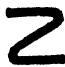
\includegraphics[keepaspectratio]{images/part002_764ec905.jpg}}

把“群”换成“环”、“子群”换成“理想”（左理想或右理想），就得到类似的结果；关于模与代数的类似结果，我们留给读者去陈述。

